% FSB Seminar — Sveučilište u Zagrebu, Fakultet strojarstva i brodogradnje
% Stereo korelacija digitalne slike — Ivan Noršić

\documentclass[12pt,a4paper]{article}

% --- Encoding, Font & Language (dual-engine) ---
\usepackage{iftex}
\ifPDFTeX
  \usepackage[utf8]{inputenc}
  \usepackage[T1]{fontenc}
  \usepackage{newtxtext}
\else
  \usepackage{fontspec}
  \setmainfont{texgyretermes-regular.otf}[
    BoldFont       = texgyretermes-bold.otf,
    ItalicFont     = texgyretermes-italic.otf,
    BoldItalicFont = texgyretermes-bolditalic.otf
  ]
\fi
\usepackage[croatian]{babel}

% --- Layout ---
\usepackage[top=2.5cm,bottom=2.5cm,left=2.5cm,right=2.5cm]{geometry}
\usepackage{setspace}
\onehalfspacing

% --- Headers & Footers ---
\usepackage{fancyhdr}
\setlength{\headheight}{13.6pt}
\pagestyle{fancy}
\fancyhf{}
\fancyhead[L]{}
\fancyhead[R]{\small\itshape \seminartitleshort}
\fancyfoot[L]{\small\itshape Fakultet strojarstva i brodogradnje}
\fancyfoot[R]{\small\itshape\thepage}
\renewcommand{\headrulewidth}{0.4pt}
\renewcommand{\footrulewidth}{0.4pt}

% --- Section Formatting (14pt Bold Uppercase) ---
\usepackage{titlesec}
\newcommand{\sectionbreak}{\clearpage}
\titleformat{\section}
  {\normalfont\fontsize{14}{17}\bfseries\MakeUppercase}
  {\thesection.}{0.5em}{}
\titleformat{\subsection}
  {\normalfont\fontsize{12}{15}\bfseries}
  {\thesubsection.}{0.5em}{}
\titleformat{\subsubsection}
  {\normalfont\fontsize{12}{15}\bfseries\itshape}
  {\thesubsubsection.}{0.5em}{}

% --- Figures & Tables ---
\usepackage{graphicx}
\graphicspath{{figures/}}
\usepackage{booktabs}
\usepackage{tabularx}
\usepackage{array}
\usepackage{float}
\usepackage{caption}
\captionsetup[figure]{font={small,bf},labelsep=period,position=below}
\captionsetup[table]{font={small,bf},labelsep=period,position=above}

% --- Numbering by section ---
\usepackage{chngcntr}
\counterwithin{figure}{section}
\counterwithin{table}{section}
\counterwithin{equation}{section}

\setcounter{secnumdepth}{4}
\setcounter{tocdepth}{4}

% --- Croatian names ---
\addto\captionscroatian{%
  \renewcommand{\figurename}{Slika}%
  \renewcommand{\tablename}{Tablica}%
  \renewcommand{\contentsname}{\normalfont\fontsize{14}{17}\bfseries SADRŽAJ}%
  \renewcommand{\refname}{\normalfont\fontsize{14}{17}\bfseries Literatura}%
}

% --- References, links, math ---
\usepackage{cite}
\usepackage[hidelinks,unicode]{hyperref}
\usepackage{amsmath}
\usepackage{amssymb}
\usepackage{xcolor}
\usepackage{tikz}
\usetikzlibrary{arrows.meta,positioning,calc}

\usepackage{indentfirst}
\setlength{\parindent}{1.25cm}
\setlength{\parskip}{0pt}

% ============================================================
% DOCUMENT METADATA
% ============================================================
\newcommand{\univname}{SVEUČILIŠTE U ZAGREBU}
\newcommand{\facultyname}{FAKULTET STROJARSTVA I BRODOGRADNJE}
\newcommand{\coursename}{FOTOGRAMETRIJA I VIZUALIZACIJA OBJEKATA}
\newcommand{\seminartitle}{Stereo korelacija digitalne slike -- mjerenje ravninskih i izvanravninskih pomaka na površini}
\newcommand{\seminartitleshort}{Stereo korelacija digitalne slike}
\newcommand{\professorname}{Izv. prof. dr. sc. Zvonimir Tomičević}
\newcommand{\authorname}{Ivan Noršić}
\newcommand{\locationdate}{Zagreb, 2026.}

% ============================================================
\begin{document}

% ---- TITLE PAGE ----
\begin{titlepage}
  \centering
  {\fontsize{14}{17}\selectfont \univname \par}
  {\fontsize{14}{17}\selectfont \facultyname \par}
  \vfill
  {\fontsize{24}{30}\bfseries \coursename \par}
  \vspace{0.8cm}
  {\fontsize{14}{18}\bfseries \seminartitle \par}
  \vfill
  \begin{tabular}{p{0.55\textwidth}>{\raggedleft\arraybackslash}p{0.35\textwidth}}
    \textmd{Nastavnici:} & \textmd{Studenti:} \\[0.3cm]
    \textbf{Izv. prof. dr. sc. Zvonimir Tomičević, mag. ing.} & \textbf{Marko Bakotić} \\
    \textbf{Dr. sc. Andrija Zaplatić, mag. ing.} & \textbf{Tin Dolenčić} \\
    \textbf{Borna Božović, mag. ing. mech.} & \textbf{Lucijan Fišter} \\
    & \textbf{Krešimir Hartl} \\
    & \textbf{Ivan Noršić} \\
    & \textbf{Matija Pongračić}
  \end{tabular}
  \vspace{1.5cm}
  \par
  {\normalfont \locationdate \par}
\end{titlepage}

% ---- FRONTMATTER ----
\pagenumbering{Roman}
\setcounter{page}{1}
\tableofcontents
\clearpage
\listoffigures
\clearpage
\listoftables
\clearpage

% ---- BODY ----
\pagenumbering{arabic}
\setcounter{page}{1}

\section{Uvod}

Mjerenje pomaka i deformacija na površini opterećenih konstrukcijskih elemenata
temeljni je zadatak eksperimentalne mehanike. Klasične mjerne metode, poput
tenzometarskih traka, daju informaciju samo u pojedinačnim točkama i zahtijevaju
fizički kontakt s uzorkom. Optičke, bezkontaktne metode -- prije svega
\emph{korelacija digitalne slike} (engl. \textit{Digital Image Correlation}, DIC)
-- omogućuju mjerenje cijelog polja pomaka i deformacija na površini uzorka bez
kontakta, uz visoku prostornu razlučivost.

Dvodimenzijska (2D) korelacija digitalne slike koristi jednu kameru i pretpostavlja
da se gibanje odvija u ravnini paralelnoj s ravninom senzora. Ta pretpostavka
narušava se čim se pojavi izvanravninski pomak: površina koja se približava ili
udaljava od kamere, savija ili rotira, unosi prividnu deformaciju koju 2D metoda
ne može razlučiti od stvarne. \emph{Stereo korelacija digitalne slike}
(stereo-DIC ili 3D-DIC) rješava taj problem korištenjem dviju kalibriranih kamera:
kombinacijom stereovizije i korelacije rekonstruira se \emph{trodimenzijsko} polje
pomaka, uključujući i ravninske i izvanravninske komponente.

\subsection{Cilj rada}

Cilj ovog seminarskog rada jest razviti funkcionalan sustav za mjerenje
trodimenzijskih pomaka i deformacija površine objekta pomoću stereo korelacije
digitalne slike, u skladu s postavljenim zadatkom. Konkretno, potrebno je:
\begin{itemize}
  \item postaviti i kalibrirati stereovizijski sustav (dvije kamere);
  \item provesti korelaciju referentne i deformiranih slika za svaku kameru;
  \item rekonstruirati trodimenzijske pomake točaka na površini uzorka;
  \item odrediti pripadno polje deformacija te vizualizirati deformirano stanje.
\end{itemize}

\subsection{Struktura rada}

U poglavlju \ref{sec:teorija} iznesena je teorijska podloga: model kamere,
projekcijske matrice, princip korelacije te stereo triangulacija. Poglavlje
\ref{sec:metoda} opisuje primijenjenu metodologiju i eksperimentalni postav, a
poglavlje \ref{sec:implementacija} programsku implementaciju u MATLAB-u.
Rezultati mjerenja na stvarnom vlačnom pokusu prikazani su i raspravljeni u
poglavlju \ref{sec:rezultati}, nakon čega slijedi zaključak.

\section{Teorijska osnova}
\label{sec:teorija}

\subsection{Korelacija digitalne slike}

Metoda korelacije digitalne slike temelji se na praćenju pomaka
nasumičnog kontrastnog uzorka (engl. speckle pattern),
koji se prije mjerenja nanosi na površinu uzorka, kroz niz slika
snimljenih tijekom deformacije.
Ako je $f(\mathbf{x})$
intenzitet referentne slike u pikselu $\mathbf{x}=(x,y)$,
a $g(\mathbf{x})$ razina
deformirane slike, uz pretpostavku očuvanja intenziteta,
materijalna točka koja se u
referentnom stanju nalazi u $\mathbf{x}$ pomiče se u deformiranom stanju u
$\mathbf{x}+\mathbf{u}(\mathbf{x})$. Tada vrijedi:
\begin{equation}
  f(\mathbf{x}) = g\big(\mathbf{x}+\mathbf{u}(\mathbf{x})\big).
  \label{eq:opt-flow}
\end{equation}
Polje pomaka $\mathbf{u}$ određuje se minimizacijom kvadratnog reziduala intenziteta piksela:
\begin{equation}
  \boldsymbol{\Phi}^2 = \sum_{\mathbf{x}\in\text{ROI}}
  \big[ f(\mathbf{x}) - g(\mathbf{x}+\mathbf{u}(\mathbf{x})) \big]^2 .
  \label{eq:dic-functional}
\end{equation}
U globalnom pristupu korelacije, korištenom u ovom radu, polje pomaka
diskretizira se mrežom konačnih elemenata, dakle pomak unutar elementa interpolira se
funkcijama oblika $N_i$ iz čvornih vrijednosti $\mathbf{u}_i$:
$\mathbf{u}(\mathbf{x})=\sum_i N_i(\mathbf{x})\,\mathbf{u}_i$. Minimizacija
\eqref{eq:dic-functional} tada vodi na linearizirani (Gauss-Newtonov) sustav koji se
rješava iterativno \cite{sutton2009}\cite{hild2006}.

\subsection{Model kamere i projekcijska matrica}

Projekcija točke prostora na ravninu senzora opisuje se tzv. \textit{pinhole} modelom.
Točka $\mathbf{X}=(X,Y,Z)$ u globalnom koordinatnom sustavu
preslikava se u piksel $\mathbf{x}=(x,y)$ preko projekcijske matrice
$\mathsf{P}\in\mathbb{R}^{3\times4}$ u homogenim koordinatama:
\begin{equation}
  s\begin{bmatrix} x \\ y \\ 1 \end{bmatrix}
  = \mathsf{P}\begin{bmatrix} X \\ Y \\ Z \\ 1 \end{bmatrix},
  \qquad
  \mathsf{P} = \mathsf{K}\,[\,\mathsf{R}\ |\ \mathbf{t}\,],
  \label{eq:projection}
\end{equation}
gdje je $s$ skalirni faktor, a $[\mathsf{R}\,|\,\mathbf{t}]$ označava matricu vanjskih (ekstriničnih) parametara kamere koja opisuje rotaciju $\mathsf{R}$ i translaciju $\mathbf{t}$ iz globalnog u koordinatni sustav kamere.

Matrica $\mathsf{K}\in\mathbb{R}^{3\times3}$ predstavlja matricu unutarnjih (intrinzičnih)
parametara kamere, definira se kao:
\begin{equation}
  \mathsf{K} = \begin{bmatrix} f_x & \alpha & c_x \\ 0 & f_y & c_y \\ 0 & 0 & 1 \end{bmatrix},
  \label{eq:intrinsic-matrix}
\end{equation}
gdje su:
\begin{itemize}
  \item $f_x$ i $f_y$ žarišne duljine kamere izražene u pikselima duž horizontalne ($x$) i vertikalne ($y$) osi slikovne ravnine,
  \item $c_x$ i $c_y$ koordinate glavne točke (engl. \textit{principal point}), koja predstavlja sjecište optičke osi kamere i ravnine senzora,
  \item $\alpha$ koeficijent iskošenosti (engl. \textit{skew coefficient}), koji opisuje odstupanje od okomitosti između osi piksela na senzoru (za moderne senzore ova se vrijednost uzima kao nula).
\end{itemize}
Kalibracijom stereovizijskog sustava određuju se projekcijske matrice obiju kamera, $\mathsf{P}_1$ i $\mathsf{P}_2$.

\subsection{Stereo triangulacija}

Ako je poznat piksel $\mathbf{x}_1$ u prvoj i pripadni piksel $\mathbf{x}_2$ u drugoj
kameri, trodimenzijska točka $\mathbf{X}$ rekonstruira se metodom triangulacije. Iz
\eqref{eq:projection} za svaku kameru vrijedi $\mathbf{x}_c \times (\mathsf{P}_c
\tilde{\mathbf{X}})=\mathbf{0}$, što daje po dvije linearne jednadžbe. Slaganjem
jednadžbi obiju kamera dobiva se homogeni sustav
\begin{equation}
  \mathsf{A}\,\tilde{\mathbf{X}} = \mathbf{0}, \qquad
  \mathsf{A} =
  \begin{bmatrix}
    x_1\,\mathbf{p}_1^{3} - \mathbf{p}_1^{1} \\
    y_1\,\mathbf{p}_1^{3} - \mathbf{p}_1^{2} \\
    x_2\,\mathbf{p}_2^{3} - \mathbf{p}_2^{1} \\
    y_2\,\mathbf{p}_2^{3} - \mathbf{p}_2^{2}
  \end{bmatrix},
  \label{eq:dlt}
\end{equation}
gdje je $\mathbf{p}_c^{k}$ $k$-ti redak matrice $\mathsf{P}_c$. Rješenje
$\tilde{\mathbf{X}}$ je desni singularni vektor matrice $\mathsf{A}$ koji odgovara
najmanjoj singularnoj vrijednosti (metoda \textit{Direct Linear Transformation}, DLT)
\cite{hartley2004}.

\subsection{Deformacije na površini}

Iz trodimenzijskog polja pomaka određuju se deformacije. Za svaki trokutasti element
konstruira se lokalni ortonormirani tangencijalni sustav, u kojem se računa gradijent
deformiranja $\mathsf{F}$ te Green-Lagrangeov tenzor deformacije
\begin{equation}
  \mathsf{E} = \tfrac{1}{2}\big(\mathsf{F}^{\mathsf{T}}\mathsf{F} - \mathsf{I}\big).
  \label{eq:green-lagrange}
\end{equation}
Iz komponenti $\mathsf{E}$ dobivaju se glavne deformacije $E_{1,2}$ te ekvivalentna
(von Misesova) deformacija, koje opisuju lokalno deformacijsko stanje površine.

\section{Metodologija}
\label{sec:metoda}

\subsection{Eksperimentalni postav}

Mjerenje je provedeno na stereovizijskom sustavu sastavljenom od dviju kamera
usmjerenih prema površini ispitnog uzorka pod kutom (Slika \ref{fig:overlay}).
Uzorak je vlačna epruveta s reduciranim mjernim presjekom, čija je mjerna površina
zakrivljena (vidljivo iz rekonstruiranog oblika na Slici \ref{fig:dispmag}); mjerna
zona prethodno je pripremljena nanošenjem nasumične crno-bijele teksture nužne za
korelaciju. Tijekom pokusa obje su kamere snimile po 1188 vremenski usklađenih slika,
od kojih prva odgovara nedeformiranom (referentnom) stanju, a ostale rastućim razinama
deformacije. U ovom je radu analizirano prvih 300 deformacijskih stanja.

\subsection{Kalibracija i geometrijski model}

Stereovizijski sustav kalibriran je unaprijed, čime su određene projekcijske matrice
obiju kamera $\mathsf{P}_1$ i $\mathsf{P}_2$ te trodimenzijska mreža konačnih
elemenata $\mathsf{M}$ koja opisuje referentni oblik mjerne površine (252 čvora, 438
trokutastih elemenata). Ispravnost kalibracije provjerena je projiciranjem čvorova 3D
mreže u obje kamere prema \eqref{eq:projection}; kao što pokazuje Slika
\ref{fig:overlay}, projicirana mreža precizno prekriva teksturiranu mjernu zonu u obje
slike, čime je potvrđena geometrijska konzistentnost sustava.

\begin{figure}[H]
  \centering
  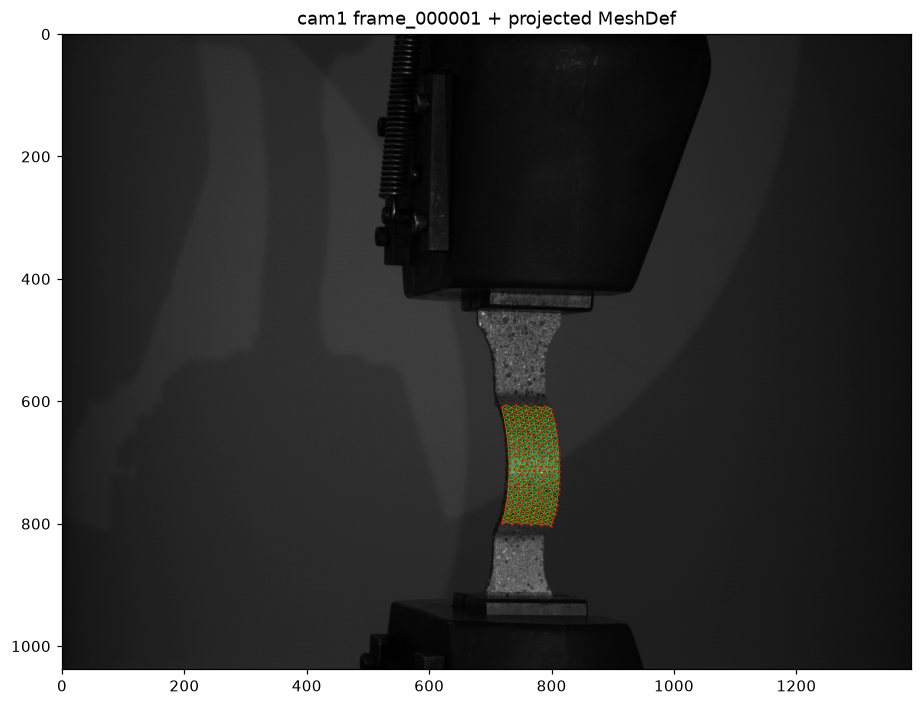
\includegraphics[width=0.49\textwidth]{overlay_cam1.png}
  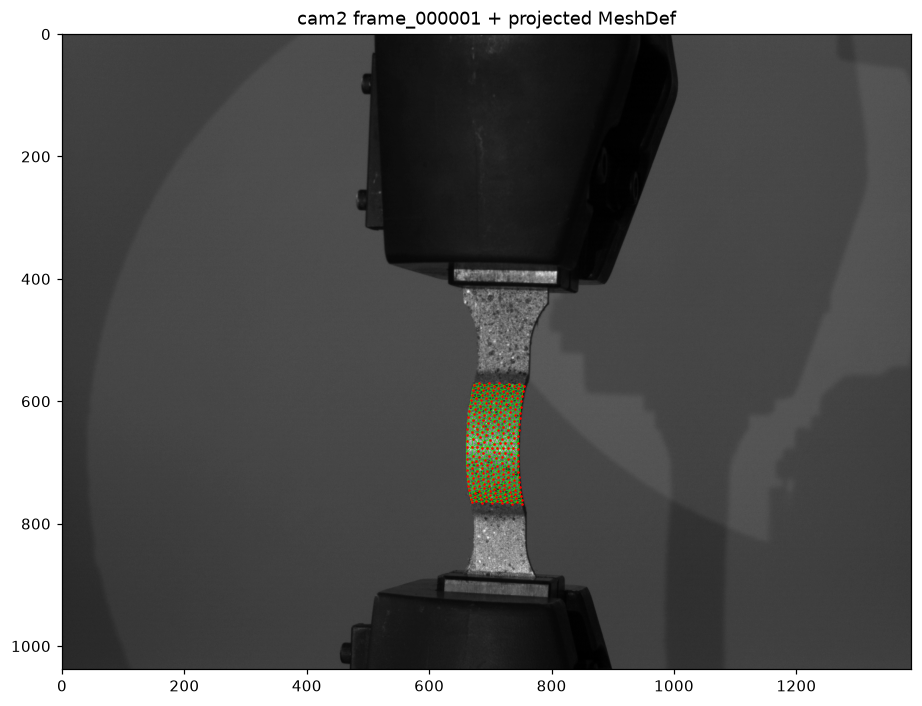
\includegraphics[width=0.49\textwidth]{overlay_cam2.png}
  \caption{Provjera kalibracije: 3D mreža projicirana matricama $\mathsf{P}_1$ (kamera
  1, lijevo) i $\mathsf{P}_2$ (kamera 2, desno) na referentnu sliku. Mreža prekriva
  teksturiranu mjernu zonu epruvete.}
  \label{fig:overlay}
\end{figure}

\subsection{Postupak mjerenja}

Primijenjeni postupak stereo korelacije provodi se u sljedećim koracima:
\begin{enumerate}
  \item \textbf{2D korelacija po kameri.} Za svaku kameru zasebno provodi se globalna
  korelacija konačnih elemenata između referentne i svake deformirane slike, čime se
  dobiva polje ravninskih (2D) pomaka čvorova mreže $\mathbf{U}_1$ i $\mathbf{U}_2$.
  \item \textbf{Korespondencija čvorova.} Budući da su obje slikovne mreže projekcije
  iste 3D mreže $\mathsf{M}$, korespondencija čvorova između kamera je zajamčena po
  konstrukciji -- čvor $i$ u kameri 1 odgovara čvoru $i$ u kameri 2.
  \item \textbf{Stereo triangulacija.} Za svaki frame i svaki čvor rekonstruira se 3D
  položaj triangulacijom \eqref{eq:dlt} iz njegovih deformiranih položaja u objema
  kamerama. Referentni 3D oblik dobiva se triangulacijom nedeformiranih položaja.
  \item \textbf{Polje 3D pomaka.} Trodimenzijski pomak čvora jednak je razlici
  trianguliranog deformiranog i referentnog položaja,
  $\mathbf{U}^{\text{3D}} = \mathbf{X}^{\text{def}} - \mathbf{X}^{\text{ref}}$.
  \item \textbf{Deformacije.} Iz polja 3D pomaka računaju se površinske deformacije
  \eqref{eq:green-lagrange} po elementu.
\end{enumerate}

Ovakav pristup -- 2D korelacija po kameri praćena triangulacijom -- omogućuje
izravno ponovno korištenje postojećeg, provjerenog algoritma 2D korelacije, uz
minimalnu dodatnu programsku logiku za stereo rekonstrukciju.

\section{Programska implementacija}
\label{sec:implementacija}

Sustav je implementiran u programskom paketu MATLAB. Vodeće načelo implementacije
bilo je ponovno korištenje postojećih, provjerenih komponenti i oslanjanje na
ugrađene MATLAB funkcije, čime je količina novoga koda svedena na najmanju mjeru.

\subsection{Ponovno korištene komponente}

Korak 2D korelacije po kameri (Poglavlje \ref{sec:metoda}) proveden je postojećim
algoritmom globalne korelacije konačnih elemenata. Rezultat -- polja čvornih 2D
pomaka za obje kamere kroz svih 300 obrađenih deformacijskih stanja -- korišten je
kao ulaz u stereo rekonstrukciju.

\subsection{Nove komponente}

Dodane su tri kratke programske jedinice, prikazane u Tablici \ref{tab:moduli}.
Triangulacija je izvedena metodom DLT preko ugrađene funkcije za dekompoziciju na
singularne vrijednosti (\texttt{svd}), a vizualizacija ugrađenim funkcijama
\texttt{trisurf} i \texttt{patch}.

\begin{table}[H]
  \centering
  \caption{Nove programske jedinice modula \texttt{Stereo3DDIC}.}
  \label{tab:moduli}
  \begin{tabularx}{\textwidth}{lX}
    \toprule
    \textbf{Datoteka} & \textbf{Uloga} \\
    \midrule
    \texttt{stereoTriangulate.m} & Linearna (DLT) triangulacija točaka iz dviju
      kamera prema \eqref{eq:dlt}. \\
    \texttt{surfaceStrains.m} & Green--Lagrangeove površinske deformacije po elementu
      prema \eqref{eq:green-lagrange}. \\
    \texttt{StereoDIC3D.m} & Glavna skripta: učitavanje podataka, triangulacija po
      frameovima, deformacije, spremanje i vizualizacija. \\
    \bottomrule
  \end{tabularx}
\end{table}

\subsection{Provjera ispravnosti}

Ispravnost implementacije potvrđena je na dva načina. Prvo, triangulacija referentnih
(nedeformiranih) položaja rekonstruira zadanu 3D mrežu s pogreškom reda veličine
$10^{-15}$, tj. do strojne preciznosti, čime je potvrđena ispravnost triangulacijskog
postupka i orijentacije projekcijskih matrica. Drugo, srednja reprojekcijska pogreška
trianguliranih deformiranih točaka iznosi približno $0{,}2$ piksela (subpikselno), što
potvrđuje ispravno pridruživanje komponenti pomaka i visoku kvalitetu korelacije.

\section{Rezultati i rasprava}
\label{sec:rezultati}

Postupak je primijenjen na 300 deformacijskih stanja vlačnog pokusa. U nastavku su
prikazani rekonstruirano polje 3D pomaka, njegove komponente, evolucija pomaka kroz
pokus te polje površinskih deformacija, uz raspravu točnosti. Svi rezultati
uključuju čišćenje rubnih čvorova opisano u odjeljku \ref{ssec:ciscenje}.

\subsection{Polje trodimenzijskih pomaka}

Slika \ref{fig:dispmag} prikazuje deformirani oblik mjerne površine obojen iznosom
ukupnog 3D pomaka. Rekonstruirana površina jasno je zakrivljena, čime se potvrđuje da
mjerenje obuhvaća i izvanravninsku komponentu koju 2D korelacija ne bi mogla razlučiti.
Polje pomaka mijenja se glatko po površini, bez naglih diskontinuiteta, što upućuje na
konzistentnost rekonstrukcije; blaga neravnost uz sam rub zone odgovara preostaloj
(subpikselnoj) mjernoj nesigurnosti rubnih elemenata.

\begin{figure}[H]
  \centering
  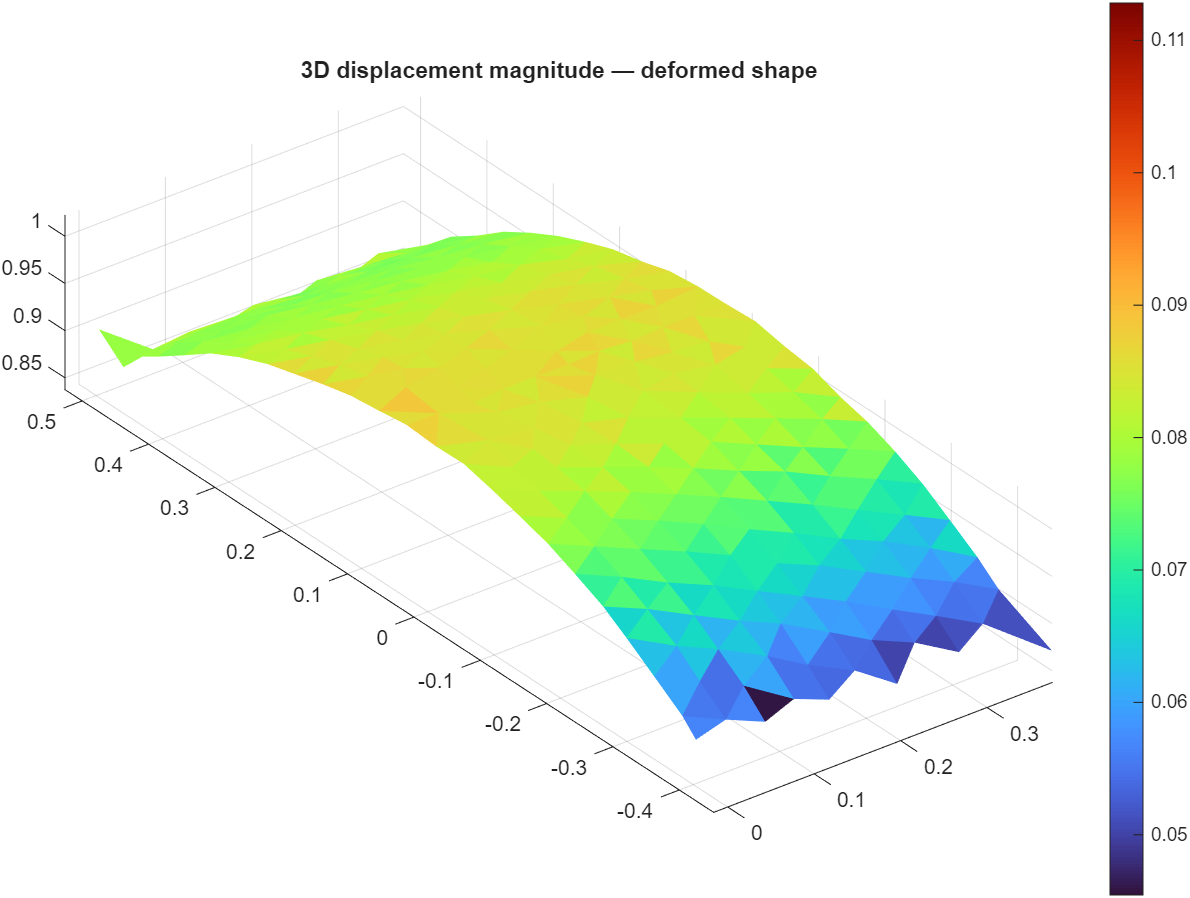
\includegraphics[width=0.78\textwidth]{disp_magnitude.png}
  \caption{Deformirani 3D oblik mjerne površine obojen iznosom ukupnog pomaka
  $|\mathbf{U}|$ (mjerne jedinice kalibracije), za posljednje deformacijsko stanje.}
  \label{fig:dispmag}
\end{figure}

Razlaganje pomaka na komponente (Slika \ref{fig:dispcomp}) daje jasniju fizikalnu
sliku gibanja. Komponenta $U_x$ (uzduž kraće osi mjerne zone) praktički je
zanemariva. Ravninsko gibanje gotovo u cijelosti nosi komponenta $U_y$, pozitivna i
približno jednolika po površini, što odgovara vlačnom razvlačenju uzorka u smjeru
osi $y$ uz pomak mjerne zone kao cjeline. Izvanravninska komponenta $U_z$ posvuda je
negativna -- cijela se površina tijekom pokusa pomiče prema kamerama odnosno
,,spljošćuje``, s najvećim iznosom na zakrivljenijem dijelu zone. Upravo ta
kombinacija (usporedivi $U_y$ i $U_z$) čini uzorak reprezentativnim testom stereo
metode: jednokamerna 2D korelacija interpretirala bi izvanravninski pomak kao lažnu
ravninsku deformaciju.

\begin{figure}[H]
  \centering
  
\includegraphics[width=\textwidth]{disp_components.png}
  \caption{Komponente 3D pomaka $U_x$, $U_y$ i $U_z$ za posljednje deformacijsko
  stanje, na zajedničkoj divergentnoj skali (kalibracijske jedinice). Ravninsko
  gibanje dominantno nosi $U_y$, a izvanravninsko $U_z$.}
  \label{fig:dispcomp}
\end{figure}

\subsection{Evolucija pomaka}

Slika \ref{fig:evolution} prikazuje najveći ukupni pomak $|\mathbf{U}|$ i najveću
izvanravninsku komponentu $|U_z|$ kroz niz frameova. Prvih tridesetak frameova čini
plato na razini $\approx 0{,}003$ kalibracijskih jedinica: uzorak još nije značajno
opterećen pa izmjerene vrijednosti predstavljaju efektivnu razinu šuma mjernog
lanca. Nakon platoa obje krivulje rastu monotono i približno linearno, uz blago
ubrzanje pri kraju pokusa (nagib u završnom dijelu $1{,}21$ puta veći od nagiba u
sredini pokusa). Vrijedi istaknuti da je prije čišćenja rubnih čvorova krivulja
pokazivala prividno naglo ubrzanje oko 240.\ framea -- ono se pokazalo artefaktom
dekorelacije čvorova 110 i 229 (Slika \ref{fig:detekcija}), a ne stvarnim ponašanjem
uzorka. U posljednjem stanju najveći ukupni pomak iznosi približno $0{,}09$, a
najveća izvanravninska komponenta $0{,}08$ (u mjernim jedinicama kalibracije) --
izvanravninski je pomak dakle gotovo jednak ravninskom, što potvrđuje nužnost stereo
mjerenja za ovakav uzorak.

\begin{figure}[H]
  \centering
  
\includegraphics[width=0.80\textwidth]{disp_evolution.png}
  \caption{Evolucija najvećeg ukupnog pomaka $|\mathbf{U}|$ i najveće izvanravninske
  komponente $|U_z|$ kroz deformacijska stanja.}
  \label{fig:evolution}
\end{figure}

\subsection{Polje deformacija}

Slika \ref{fig:strain} prikazuje polje glavne deformacije $E_1$ po površini u
posljednjem stanju. Tipična (medijalna) vrijednost glavne deformacije iznosi približno
2\,\% ($1{,}95\,\%$), što je red veličine očekivan za vlačni pokus metalnog uzorka u
elastično-plastičnom području. Deformacija računata po elementu pokazuje razinu šuma
svojstvenu deriviranju polja pomaka na linearnim trokutastim elementima; skala boja
stoga je ograničena robusnim 97.\ percentilom ($12{,}04\,\%$). Nakon čišćenja rubnih
čvorova najveća vrijednost po elementu iznosi $27{,}36\,\%$ (prije čišćenja
nefizikalnih $328{,}69\,\%$); preostale povišene vrijednosti uz rub zone odraz su
subpikselne nesigurnosti rubnih elemenata koja se deriviranjem pojačava, a mogle bi
se dodatno smanjiti zaglađivanjem (ekstrapolacijom deformacija u čvorove) ili
profinjenjem mreže.

\begin{figure}[H]
  \centering
  
\includegraphics[width=0.78\textwidth]{strain_E1.png}
  \caption{Polje glavne (najveće) deformacije $E_1$ na rekonstruiranoj 3D površini.}
  \label{fig:strain}
\end{figure}

\subsection{Procjena točnosti}
\label{ssec:tocnost}

Točnost sustava ocijenjena je posredno, kroz tri neovisna pokazatelja. Prvo,
rekonstrukcija referentnog oblika podudara se sa zadanom mrežom do strojne
preciznosti ($\sim 10^{-15}$), čime je isključena sustavna pogreška triangulacije.
Drugo, srednja reprojekcijska pogreška trianguliranih deformiranih točaka iznosi
približno $0{,}15$ piksela (medijan $0{,}13$ px, najveća $1{,}10$ px) -- budući da ta
veličina objedinjuje pogrešku korelacije, kalibracije i triangulacije, subpikselna
vrijednost potvrđuje visoku ukupnu točnost mjerenja i u razini je vrijednosti koje
se u literaturi navode za dobro kalibrirane stereo-DIC sustave. Treće, plato
krivulje evolucije u neopterećenom dijelu pokusa daje procjenu šuma pomaka od
$\approx 0{,}003$ kalibracijskih jedinica.

Lokalizirani gubitak korelacije na tri rubna čvora kamere 2, koji je prije čišćenja
bio dominantan izvor pogreške (reprojekcija do $6{,}25$ px, nefizikalni ekstremi
deformacija), automatski je detektiran i saniran postupkom iz odjeljka
\ref{ssec:ciscenje}. Preostala nesigurnost svodi se na šum polja deformacija po
elementu, koji se po potrebi može dodatno smanjiti zaglađivanjem ili profinjenjem
mreže uz rub.

\section{Zaključak}

U radu je razvijen i primijenjen funkcionalan sustav za mjerenje trodimenzijskih
pomaka i deformacija površine objekta pomoću stereo korelacije digitalne slike.
Primijenjen je pristup koji spaja globalnu 2D korelaciju konačnih elemenata po svakoj
kameri sa stereo triangulacijom čvorova mreže, čime je uz minimalnu količinu novoga
koda ostvarena potpuna 3D rekonstrukcija.

Sustav je uspješno primijenjen na stvarni vlačni eksperiment 3D tiskane polimerne
epruvete s 300 deformacijskih stanja. Svi su rezultati, uz pomoć mjerila slike od
$0{,}0502$\,mm/px i iz njega izvedenog mjerila prostora, izraženi u fizikalnim
jedinicama. Rekonstruirana su glatka polja trodimenzijskih pomaka, jasno
obuhvaćajući i ravninske
i izvanravninske komponente. U posljednjem stanju najveći ukupni pomak iznosi
$0{,}97$\,mm, a najveća izvanravninska komponenta $0{,}87$\,mm, dakle izvanravninski
pomak gotovo je jednak ravninskom. Pripadna polja površinskih deformacija pokazuju
medijalnu glavnu deformaciju od približno 2\,\%.

Mjerna nesigurnost sustava određena je izravno iz 20 slika neopterećenog uzorka.
Standardna nesigurnost pomaka iznosi $2{,}57\cdot10^{-3}$\,mm ($0{,}05$\,px) za
kameru 1, odnosno $3{,}40\cdot10^{-3}$\,mm ($0{,}07$\,px) za kameru 2, uz
nesigurnost deformacija reda veličine $10^{-3}$. Analiza ovisnosti nesigurnosti
o veličini elementa potvrdila je da je odabrana mreža nominalne veličine $10$\,px
povoljan kompromis razlučivosti i šuma, a ispravnost implementacije potvrđena je
rekonstrukcijom referentnog oblika do
strojne preciznosti i subpikselnom reprojekcijskom pogreškom ($\approx 0{,}15$\,px).
Lokalizirani gubitak korelacije na tri rubna čvora jedne kamere automatski je
detektiran usporedbom sa susjednim čvorovima i saniran robusnim medijalnim filtrom,
bez utjecaja na ostatak mjernog polja i bez izmjena mjernih algoritama.

Time su ispunjeni svi ciljevi zadatka. Postavljen je stereovizijski model
(kalibriran ChArUco pločom), provedena
korelacija između referentnih i deformiranih slika, izračunati 3D pomaci i
deformacije u stvarnim jedinicama, određena mjerna nesigurnost te vizualizirano
deformirano stanje. Mogući smjerovi daljnjeg rada
uključuju izglađivanje polja deformacija ekstrapolacijom u čvorove, profinjenje mreže
uz rub mjerne zone te inkrementalnu strategiju korelacije (ažuriranje referentne
slike) kojom bi se analiza proširila i na preostala deformacijska stanja do loma.


% ---- LITERATURA ----
\clearpage
\addcontentsline{toc}{section}{Literatura}
\bibliographystyle{unsrt}
\bibliography{references}

\end{document}
